\documentclass[letterpaper, 12pt]{article}
\usepackage[margin=1in]{geometry}
\usepackage{amsmath}
\usepackage{pgfplots}
\usepackage{listings}
\usepackage{graphicx}
\usepackage{amsmath}
\usepackage{amssymb}
\usepackage{amsthm}
\pgfplotsset{width=15cm,compat=1.9} \newcommand{\todo}[1]{{\emph{\color{red}#1}}}
\title{WIP: The Optimization of Alcoholism under a Hypothetical Bartering System}
\author{Kevin Palani and Kevin Zheng}
\begin{document}
\maketitle
\tableofcontents
\lstset{
    breaklines=true
}
\section{Introduction to the hypothetical bartering system}
\par You have \$10, and a beer is 2\$.
Very quickly you can see that if you spend all 10\$, you will get 5 beers.
Once you've drunken the 5 beers, you are left with 5 beer bottles and 5 caps.
The store owner strikes you a deal.
If you give him two empty bottles or four bottle caps, he'll give you a new bottle of beer.
He is also kind enough to let you drink before you pay, but you are not allowed to be in bottle or cap-debt.
How many drinks you can get?
\section{Naive solution}

\section{Modeling amount of caps and bottles}
\subsection{Vector representation of caps and bottles}
\[
    \begin{bmatrix}
        a\\
        b\\
    \end{bmatrix}
\]
\par Will be the vector that represents the bottles and caps such that $a$ is the amount of bottles, and $b$ is the amount of caps.
\subsection{Representation of the bartering system}
\par If we can spend two empty bottles and receive a full drink, that is equivalent to spending two bottles and getting one bottle and one cap.
We will represent this operation as the addition of the following vector;
\[
    \begin{bmatrix}
       -2 + 1\\
       1\\
    \end{bmatrix}
\]
\par And since we can drink before we pay, having only one empty bottle is enough to drink.
\[
    \begin{bmatrix}
       -1\\
        1\\
    \end{bmatrix}
\]
\par Using 4 caps can be represented simliarly
\[
    \begin{bmatrix}
        1\\
        -4 + 1\\
    \end{bmatrix}
\]
\par Which can simply be evaluated to.
\[
    \begin{bmatrix}
         1\\
        -3\\
    \end{bmatrix}
\]
\par These two operations can be represented geometrically as a translation of a point on a 2 dimensional Cartesian plane.
For example, if we start with 5 empty bottles and 5 empty caps, we can trace the motion of the point as following.
\begin{center}
    \begin{tikzpicture}
        \begin{axis}[
                axis lines = left,
            xlabel = Bottles,
            ylabel = {Caps},
            xmin = 0, xmax = 10,
            ymin = 0, ymax = 10
            ]
            \addplot [
                domain=0:5,
            samples=100,
            color=blue,
            ]
            {-1 * (x - 5) + 5};
            \addlegendentry{Trading empty bottles for drinks}
            \addplot [
                domain=0:3,
            samples=100,
            color=red,
            ]
            {-3 * x + 10};
            \addlegendentry{Trading caps for drinks}
            \addplot [
                domain=0:3,
            samples=100,
            color=blue,
            ]
            {-1 * (x - 3) + 1};
            \addplot [
                domain=0:1,
            samples=100,
            color=red,
            ]
            {-3 * x + 4};
            \addplot [
                domain=0:1,
            samples=100,
            color=blue,
            ]
            {-1 * (x - 1) + 1};
            \addplot[
                color=blue,
            only marks,
            mark=square,
                    ]
            coordinates {
                (0,2)(5,5)
            };
        \end{axis}
    \end{tikzpicture}
\end{center}
\section{Analysis of the graph}
Since having either 1 bottle, or 3 caps is enough to do another transaction, we know from the context of the problem, that the final state must be one of the following points:
$$(0, 0)$$
$$(0, 1)$$
$$(0, 2)$$

Visually, you can already tell that it's impossible to get to the point $(0, 0)$ unless if you have already started there (sorry mate, you gotta buy some beer to play the game).

You can also tell that you cannot get to $(0, 1)$, because that means you came from $(1, 0)$ through a blue line, but that means you came from $(0, 2)$ from a red line, which is impossible because $(0, 2)$ is not enough to continue a transaction.

So already from this graph, you can tell that you will always end up with 2 caps left over (if we ignore the trivial case that you do not buy beer in the first place).
\section{Algebraic Solution}
Let $\vec{i}$ be the initial state, $\vec{f}$ be the final state, $c$ be the number of cap-based transactions, and $b$ be the number of bottle-based transactions.
\begin{align*}
    \vec{i}
    + c
    \begin{bmatrix}
        -3\\
        1
    \end{bmatrix}
    + b
    \begin{bmatrix}
        1\\
        -1
    \end{bmatrix}
    &=
    \vec{f}\\
    c
    \begin{bmatrix}
        -3\\
        1
    \end{bmatrix}
    + b
    \begin{bmatrix}
        1\\
        -1
    \end{bmatrix}
    &=
    \vec{f} - \vec{i}\\
    \begin{bmatrix}
        -3 & 1\\
         1 &-1
    \end{bmatrix}
    \begin{bmatrix}
        c\\
        b
    \end{bmatrix}
    &=
    \vec{f} - \vec{i}\\
    \begin{bmatrix}
        c\\
        b
    \end{bmatrix}
    &=
    \frac{1}{2}
    \begin{bmatrix}
        -1 &-1\\
        -1 &-3
    \end{bmatrix}
    (\vec{f} - \vec{i})\\
\end{align*}
Initially we get the same amount of caps and bottles according to how many drinks $i$ that we start with.
\begin{align*}
    \begin{bmatrix}
        c\\
        b
    \end{bmatrix}
    &=
    \frac{1}{2}
    \begin{bmatrix}
        -1 &-1\\
        -1 &-3
    \end{bmatrix}
    (\vec{f} - \vec{i})\\
    \begin{bmatrix}
        c\\
        b
    \end{bmatrix}
    &=
    \frac{1}{2}
    \begin{bmatrix}
        1 & 1\\
        1 & 3
    \end{bmatrix}
    (\vec{i} - \vec{f})\\
    \begin{bmatrix}
        c\\
        b
    \end{bmatrix}
    &=
    \frac{1}{2}
    \begin{bmatrix}
        1 & 1\\
        1 & 3
    \end{bmatrix}
    i
    \begin{bmatrix}
        1\\
        1
    \end{bmatrix}
    -
    \frac{1}{2}
    \begin{bmatrix}
        1 & 1\\
        1 & 3
    \end{bmatrix}
    \vec{f}\\
    \begin{bmatrix}
        c\\
        b
    \end{bmatrix}
    &=
    i
    \begin{bmatrix}
        1\\
        2
    \end{bmatrix}
    -
    \frac{1}{2}
    \begin{bmatrix}
        1 & 1\\
        1 & 3
    \end{bmatrix}
    \vec{f}
\end{align*}

If we simply make $\vec{f} = \vec{0}$, then we don't reach a contradiction even though we know from looking at the graph that it's not possible.
This is because there's always a way to get to $(0, 0)$ if we choose to fall into debt, but since that's against the rules, we have to make a check that there exists a way to reach $\vec{f}$.

We can describe the validity $v$ of transaction $c$ and $b$ using the following recursive function:
\begin{align*}
    v(c, b) &= v(c - 1, b) \times v(c, b - 1) \times \underbrace{(
        \begin{bmatrix}
            -3 & 1\\
            1 & -1\\
        \end{bmatrix}
        \begin{bmatrix}
            c\\
            b
        \end{bmatrix}
        + \vec{i}
        >
        \vec{f}
    )}_\text{1 if this is true, 0 if this is false}\\
    v(0, 0) &= 1
\end{align*}

If we brute force using a script:

\lstinputlisting[language=python]{python/non-debt-transactions.py}

Then we get the following result where the green dots represents the possible transactions:
\begin{center}
    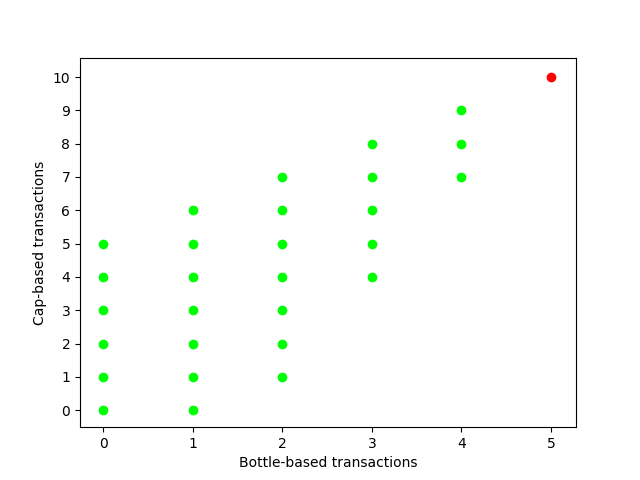
\includegraphics[width=0.75\textwidth]{python/debt.png}
\end{center}

The goal is to get as drunk as possible, which is reaching as many transactions as possible, thus we want to maximize $b + c$ with respect to the elements of $f$.
The above matrix equation can be represented as the following set of equations.
\begin{align*}
    c &= \frac{1}{2}(-(f_c - i_c) - (f_b - i_b))\\
    b &= \frac{1}{2}(-(f_c - i_c) - 3(f_b - i_b))\\
    c + b &= \frac{1}{2}(-2(f_c - i_c) - 4(f_b - i_b))
\end{align*}
Which can be simplified to:
\begin{align*}
    c &= \frac{1}{2}(-f_c - f_b  + i_c + i_b))\\
    b &= \frac{1}{2}(-f_c - 3f_b + i_c + i_b))\\
    c + b &= -f_c - 2f_b + i_c + 2i_b
\end{align*}
Using the typical optimization with derivatives isn't going to help us here, because the function is linear with respect to both $f_c$ and $f_b$.
Instead we can use the constraint that $c$, $b$, and $c + b$ must be natural numbers (in my definition, the natural numbers include 0).
\begin{align*}
    c &\in \mathbb{N} \\
    -f_c - f_b + i_b + i_c &\in 2\mathbb{N}
\end{align*}
Since $i_b = i_c$, $i_b + i_c \in 2\mathbb{N}$
\begin{align*}
    -f_c - f_b &\in 2\mathbb{Z}\\
    f_c + f_b &\in 2\mathbb{N}
\end{align*}
Thus, we can say that $f_c$ and $f_b$ have the same parity.
\section{Using the final state of the vector to deduce the amount of drinks drunk}
\par Since two empty bottles can get you a drink and a drink is worth \$2, then that means one bottle is worth \$1.
Similarly since four bottle caps can get you a drink and a drink is worth \$2, then that means bottle cap is worth \$0.5.
\par Since a full drink is consisted of one cap, one bottle, and some drink, we can use simple algebra to deduce that:
\begin{equation}
    \$2 = d + \$1 + \$0.5
\end{equation}
\begin{equation}
    d = \$0.5
\end{equation}
the worth of the drink is \$0.5.
If we started with \$10 dollars, and we are left with $a$ bottles and $b$ caps, then:
\begin{equation}
    \$10 = \$0.5x + \$a + \$0.5b
\end{equation}
\begin{equation}
    x = \frac{\$10 - \$a - \$0.5b}{\$0.5}
\end{equation}
\end{document}
